\documentclass[a4paper,12pt]{report}
\usepackage[utf8]{inputenc}
\usepackage[T1]{fontenc}
\usepackage[ngerman]{babel}
\usepackage[parfill]{parskip}
%\usepackage{eurosans}
\usepackage[top=3cm, left=3cm]{geometry}
\usepackage{setspace}
\usepackage{mdwlist}
\usepackage{graphicx}
\usepackage{eurosym}
\renewcommand*\familydefault{\sfdefault}

\setcounter{secnumdepth}{-1}

\begin{document}

\title{\textbf{Leitfaden für das ESE-Tutorium 2014 für Masterstudenten}\\}
\date{}
\author{von\\Thomas Heinze, Berit Lochner, Denis Stein (2008), \\Marcus Hähnel und Nico Hoffmann (2009), \\Marius Melzer (2010), \\Robert Schädel (2011),\\Sascha Peukert (2013), \\Kilian Költzsch, Marc Satkowski und Sascha Peukert (2014)}
\maketitle

\chapter{Hinweise für Tutoren}
\section{Ansprechpartner}
Kilian (koeltzsch@ifsr.de): 0151/41929976\\
Marc (satkowski@ifsr.de): 0172/8572425 \\
FSR/ESE-Orga (ese-orga@ifsr.de): 0351/463-38226

\section{Über das Tutorium}
\begin{itemize*}
\item Ziel des Tutoriums ist Vermittlung von Informationen rund um das Studium.
\item Der Inhalt dieser Handreichung ist das Minimum, was ihr in den Tutorien vermitteln sollt.
Ihr könnt die Stichpunkte gerne noch mit eigenen Einfällen ergänzen.
\item Die Informationen sollten möglichst \textbf{unparteiisch} und \textbf{nicht wertend} vermittelt werden.
Insbesondere sollte man vermeiden, den Erstis schon vorab Angst vor bestimmten Vorlesungen oder Dozenten zu machen oder sie zum Nichtbesuchen der Vorlesungen zu animieren.
Betrifft vor allem auch das ESE-Spiel.
%\item Eine Tutoriengruppe besteht aus zwei Tutoren und ca. 15-25 Erstis.
\item Falls keiner der beiden Tutoren zu einem Thema eine Auskunft geben kann, verweist am besten auf erfahrenere ESE-Tutoren oder den FSR, anstatt (möglicherweise falsche) Spekulationen zu äußern.
Montag Nachmittag wird das FSR-Büro besetzt sein, sodass ihr Leute mit spezifischeren Fragen auf Montag Nachmittag verweisen könnt.
\item Die Master-Gruppe hat keinen Namenspatron und keine dedizierte Evaluation. Die ESE-Tassen werden nach dem Tutorium direkt übergeben.
\end{itemize*}

\section{Vor dem Tutorium zu erledigende Dinge}
\begin{itemize*}
\item Lest euch diesen Leitfaden schon mal im Ganzen durch.
Es wäre schlecht, wenn ihr das erst im Tutorium selbst tun müsst!
Markiert euch eventuell wichtige Punkte.
Wenn ihr Fragen habt, stellt diese beim Tutorentreffen oder per Mail.
\item In der unten stehenden Tabelle Ort eures Tutoriums nachsehen.
\item Den Raum bitte vorher schonmal suchen, falls ihr nicht sicher wisst, wo er sich befindet.
\item Am ESE-Montag bitte spätestens um 9:00 da sein und mit helfen (10:00 geht die Begrüßung mit den anschließenden Tutorien los)!
Wir treffen uns in der INF/E023 zum Frühstück.
\item Am Montag um 09:30 ist in der INF/E008 ein letztes Tutorentreffen.
Dort bekommt ihr ein letztes Briefing  und die letzten Gruppen haben die Chance, Helfer zu casten.
\item Überlegt euch zusammen mit eurem Tutoriumspartner, wie ihr die Informationen vortragen wollt.
Möglicherweise wollt ihr bestimmte Dinge an die Tafel schreiben.
Vielleicht ist es am sinnvollsten, die Stichpunkte abwechselnd vorzutragen, damit der jeweils andere sich schon mal Gedanken zum nächsten machen kann.
\item Stellt euch ebenfalls darauf ein, am Dienstag zur \textbf{Übungseinschreibung} zwischen 8:40 und 12:30 Uhr anwesend zu sein und zu helfen. Die neuen Masterstudenten müssen natürlich nicht an der Einschreibung teilnehmen.
\end{itemize*}

\begin{center}
\vspace{1cm}
\begin{tabular}[h]{|l|l|l|l|}
	\hline
	\textbf{`'Namenspatron''} & \textbf{Tutor(en)} & \textbf{Raum}\\ \hline
	Master (alle) & Sascha \& Patrick & INF/E023\\
	\hline
\end{tabular}
\end{center}

\chapter{Zu vermittelnde Informationen}

\section{Einführung}
\begin{itemize*}
\item Macht eine kleine Vorstellungsrunde, um euch kennenzulernen und die Atmosphäre ein bisschen aufzulockern. Auch wenn viele der Master-Erstis ihren Bachelor in Dresden gemacht haben, ist es dennoch wichtig für die zugezogenen Erstis.
Die Tutoren beginnen.
Am besten ihr erzählt, wie ihr heißt, wo ihr ursprünglich herkommt, was euch an der (Medien-) Informatik gefällt. 
Die Studenten könnten zusätzlich noch erwähnen, was sie vorher gemacht haben und wieso sie sich für das Inf/MInf-Studium in Dresden entschieden haben.
Schreibt am besten an die Tafel, was ihr gerne von den Erstis wissen möchtet.
\item Falls ihr eurer Gruppe anbieten wollt, auch nach dem Tutorium eventuell aufkommende Fragen zu beantworten, schreibt eure Emailadressen an die Tafel.
%\item Erzählt etwas zu eurem Namenspatron. Informationen zu diesem findet ihr im Anhang.
\end{itemize*}

\section{ESE-Woche}
\begin{itemize*}
\item ESE-Website: http://ese.ifsr.de (mit aktuellem Ablaufplan der ESE-Woche (da er sich auch in der Woche noch verändern kann), Weblinks, etc.)
\item Den Zeitplan gibt es auch im iCal Format (ICS Datei) auf ese.ifsr.de zum Download.
Kann man sich direkt in den Kalender importieren.
\item Der Ablaufplan der ESE wird am FSR-Büro hinter der Wendeltreppe hängen und auf der ESE-Webseite stehen.
\item Die wichtigen Dinge der ESE-Tüte durchgehen: NoPanic, Stundenplanauswahl (betrifft Master nicht), etc.
\item Geht die ESE-Woche durch und sagt kurz etwas zu den wichtigsten Programmpunkten für Master
\end{itemize*}
\vspace{0.5cm}
Ort der Begrüßung ist der Lichtenheldt-Hörsaal im Zeunerbau (Bombentrichter) und der der Vorträge ist die ganze Woche über die INF/E023.

% TODO: Graphischer Zeitplan
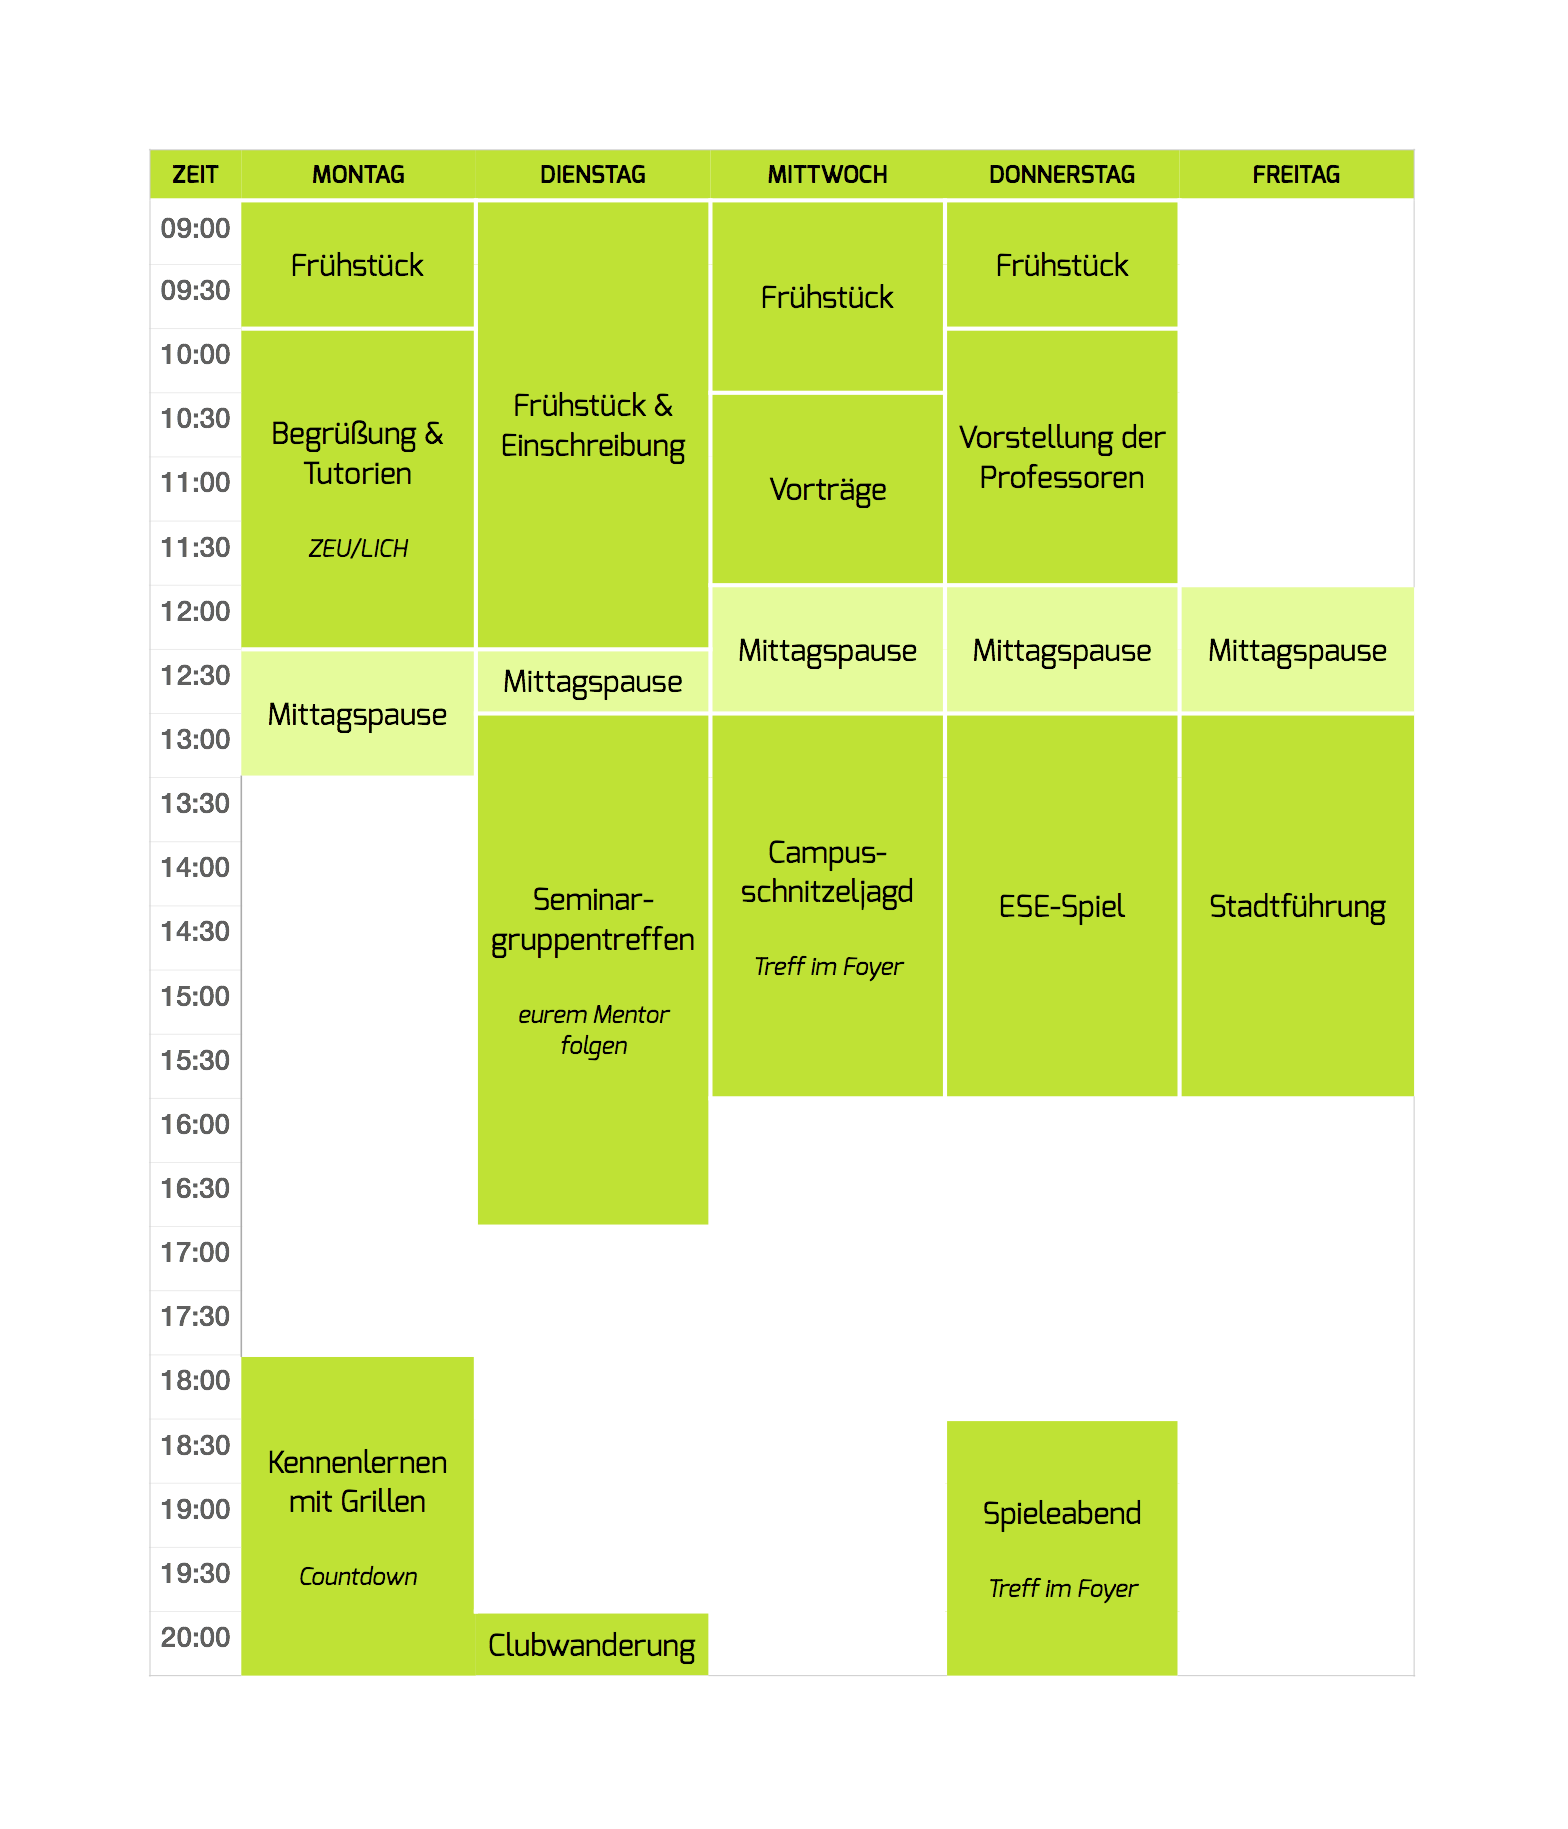
\includegraphics[width=\linewidth]{./zeitplan.png}

\subsection{Montag}
09:00 - 10:00 Frühstück\\
10:00 - 11:00 Begrüßung im ZEU/LICH\\
11:00 - 12:30 Tutorien (siehe Tabelle auf S.2)\\
Seht euch frei darin euren Erstis einen gemeinsamen Mensabesuch im Anschluss an das Tutorium anzubieten.
am Nachmittag Sprechstunde im FSR-Büro\\
Wenn ihr ausländische Studierende in eurer Gruppe habt, erinnert sie bitte an ihre Tutorien am Montag Nachmittag – sie sollten wissen, worum es geht.\\
\\
ab 18:00 Kennlernabend mit Grillen (im Studentenclub Count Down (Güntzstraße 22))\\

\subsection{Dienstag}
09:00 - 12:00 Frühstück und parallel Einschreibung (Unwichtig für Master )\\
12:30 - 13:00 Mittagspause \\
ab 13:00  Erstes Seminargruppentreffen (Unwichtig für Master )
\\
ab 20:00 Clubwanderung (Startet beim Studentenclub Count Down (Güntzstraße 22))\\
Bitte weist darauf hin, dass die Clubwanderung aus Versehen nicht im Zeitplan in der No Panic auftaucht und keinesfalls flach fällt.

\subsection{Mittwoch}
09:00 - 10:30 Frühstück\\
ab 10 Uhr Vortragsfähigkeit der E023 herstellen\\
10:30 - 11:00 Vortrag Studienangelegenheiten und Organisation  (sehr wichtig!)\\
11:00 - 11:30 Vortrag Auslandsstudium \\
11:30 - 11:45 Vortrag studentische Mitbestimmung \\
11:45 - 12:00 Vortrag TUDIAS \\
12:00 - 13:00 Mittagspause \\
12:40 Helfertreff Schnitzeljagd
13:00 - 16:00 Campus-Schnitzeljagd \\


\subsection{Donnerstag}
09:00 - 10:00 Frühstück\\
10:00 - 12:00 Vorstellung der Professoren\\
12:00 - 13:00 Mittagspause\\
12:40 Helfertreff ESE-Spiel
13:00 - 16:00 ESE-Spiel\\
\\
ab 18:30 Spieleabend in der Fakultät\\

\subsection{Freitag}
13:00 - 16:00 Stadtführung (bitte erfragt grob das Interesse und gebt es weiter an Philipp <heisig@ifsr.de>)\\

\subsection{Einschreibung}
\begin{itemize*}
	\item Einschreibung zu Veranstaltungen variiert je nach Veranstaltung.Entwerder wird jExam, Opal oder nichts genutzt.
	
	\item Optionale (aber ratsame!) Mailinglisten:
		\begin{itemize*}
		\item FSR-info ist der Verteiler des FSR über den regelmäßig Informationen zu den Vorgängen an der Fakultät und den Sitzungen des FSR kommen.
		\item extern: Jobangebote werden über diese Mailingliste verbreitet.
		\item und diverse andere,Einschreibung unter \\ https://www.ifsr.de/fsr:news:quicklinks\_fuer\_die\_einschreibung  (An die Tafel schreiben)
	\end{itemize*}
\end{itemize*}

\section{Studium}
\subsection{Allgemein}
\begin{itemize*}
	\item Alle wichtigen Informationen bezüglich des Ablaufs des Studiums befinden sich in der Prüfungs- und Studienordnung (Inf-Website -> Studium -> Für Studierende -> Regularien -> Studien- und Prüfungsordnungen).
	In den Anhängen (separate PDFs!) befindet sich jeweils eine nützliche Stundentafel mit den zu Belegenden Fächern geordnet nach Studiensemester.
	Für den Bachelor stehen gute Beschreibungen der einzelnen Module in der Studienordnung - reingucken lohnt sich.

	\item Das wissen um Module und Lehrveranstaltungsformen wird vorrausgesetzt.
	\item Prüfungen können zwei mal wiederholt werden.
	Wer durch eine Prüfung fällt, hat ein Jahr (zwei Semester) Zeit, diese zu wiederholen, für die zweite Wiederholung hat man allerdings darauf hin nur ein Semester Zeit.
	Wer die 2. WH (Wiederholungsprüfung) nicht schafft, wird exmatrikuliert und hat somit sein Studium nicht geschafft.
	\item Eine Abmeldung von einer Prüfung ist ohne Angabe von Gründen bis 3 Werktage (bzw. 2 Wochen bei mündlichen Prüfungen) vor dem Prüfungstermin möglich.
	\item Innerhalb der genannten Frist spricht man von Rücktritt.
	Ein Rücktritt ist nur bei Krankheit o.ä. zulässig und muss dem Prüfungsamt unverzüglich schriftlich mitgeteilt werden (ärztliches Attest o.ä.).
	
	\item Zu jedem Studiengang gehört ein Prüfungsausschuss.
	An diesen können Anträge auf Anerkennung bzw. Anrechnung von Studien- und Prüfungsleistungen, Anträge auf Prüfungsfristverlängerung, Anträge auf Annullierung einer Prüfung, etc. gestellt werden
	\item Man kann seine Studienzeit durch Urlaubs- und Gremiensemester verlängern.
	Ein Urlaubssemester ist ein studienfreies Semester, in dem neuerdings auch Prüfungen geschrieben werden können. 	Gremiensemester sind eine Reduzierung der Fachsemesterzahl.
	Man bekommt sie durch Engagement in den Gremien der Fakultät, z.B. als Mitglied von Fachschaftsrat, Fakultätsrat, Prüfungsausschuss, etc.
	\item Eine Zusammenstellung von fürs Studium wichtigen Dokumenten und Links zu vielen Skripten findet man auch auf der FSR-Seite (ifsr.de -> Studium).

\end{itemize*}

\subsection{Master Informatik}
\begin{itemize*}
	\item \textbf{Basismodule:} 3 von 8 sind aus folgender Liste zu wählen zu wählen
	\begin{itemize*}
		\item Angewandte Informatik 	
		\item Künstliche Intelligenz 	
		\item Software- und Web-Engineering  
		\item Systemarchitektur 	
		\item Technische Informatik 	 
		\item Theoretische Informatik 
		\item Grafische Datenverarbeitung 
		\item Anwendungsfach
	\end{itemize*}	
	\item Das Anwendungsfach entspricht einem `'kleinen'' Nebenfach
	\item Auf http://web.inf.tu-dresden.de/Fak/w/15/stundenplan.html lassen sich alle Veranstaltungen des Semesters finden (meist mit Link zur jeweiligen Veranstaltungsseite).
	\item Bei den meisten Basismodulen muss man mindestens 2 Vorlesungen und 2 Übungen belegen und die restlichen 4 SWS sind frei wählbar. Trotzdem lieber in die Modulbeschreibung schauen!
	\item Ddie gewählten Veranstaltungen in einem Basismodul werden zusammen in einer mündlichen Komplexprüfung geprüft.
	\item \textbf{Vertiefungsmodul:} Eines der Basismodule (nicht das Anwendungsfach) muss weiter vertieft werden. Der Ablauf ist analog, diesmal müssen aber 10 SWS belegt werden.
	\item \textbf{Profilmodule:} Die Veranstaltungen für die Profilmodule werden ebenfalls aus dem Katalog gewählt. Hierbei ist zu beachten dass die Module aufeinander aufbauen müssen. Wählt man eine Veranstaltung aus dem Grundlagenforschungsmodul, muss als nächstes eine Veranstaltung aus dem Katalog Forschungsprojekt Grundlagen gewählt werden. Wählt man eine Veranstaltung aus dem Anwendungsforschungsmodul, muss man als nächstes eine Veranstaltung aus dem Katalog Forschungsprojekt Anwendung wählen. In den meisten fällen umfasst das erste Modul eine Vorlesung mit Übung und das zweite Modul 1-2 Komplexpraktika. Nur das zweite Modul ist benotet.
	\item \textbf{Vertieftes Master-Praktikum:} Funktioniert analog zum 2.Profilmodul. Hier sind 8 SWS Komplexpraktika zu wählen.
	\item \textbf{Allgemeine Qualifikation:} Für dieses Modul sind Lehrveranstaltungen im Umfang von 180h zu erbringen. Dabei werden:  Sprachkurse und Vorlesungen mit 60h je 2SWS und Seminare / Workshops mit 30h je 2SWS angerechnet. 150h sind mit Angeboten anderer Fachbereiche/Fakultäten oder ausgewählten, benoteten Veranstaltungen der Fakultät Informatik (Tabelle 1) zu belegen. Dazu zählen:
	\begin{itemize*}
    		\item benotete Sprachkurse Englisch EBW F1, F2, F3 (Tudias)
    		\item benotete Sprachkurse (Tudias)
                     \item fachfremde, \textbf{benotete} Veranstaltungen im Bereich Studium Generale
	\end{itemize*}
	\item Die letzten 30h sind aus dem Angebot der Fakultät zu wählen (Hauptseminare). 
\end{itemize*}

\subsection{Master Medieninformatik}
\begin{itemize*}
	\item \textbf{Vertiefungsmodule:} 5 bzw. 6 von 10 sind aus folgender Liste zu wählen zu wählen
	\begin{itemize*}
		\item Software Engineering Ubiquitärer Systeme
		\item Multimedia Information Retrieval and Management
		\item Advanced Web-Engineering
		\item Advanced Multimedia User Interfaces
		\item Interaktionsdesign Theorie
		\item Interaktionsdesign Praxis
		\item Interaktionstechnologie für die künstlerische Praxis
		\item Basismodul Graphische Datenverarbeitung
		\item Angewandte Graphische Datenverarbeitung
		\item eLearning
		\item Multimodale Benutzungsoberflächen
	\end{itemize*}
	\item Je nach Mdoul müssen Veranstaltungen belegt werden, wie im Modulkatalog angegeben
	\item Es müssen Mdoule von insgesamt 60 LP gewählt werden, die meisten Module haben 12 LP, manche aber auch nur 6 LP
	\item Lehrveranstaltungen können oftmals in mehrere Module eingebracht werden, daher ist zu empfehlen sich vor deren Prüfung eine grundlegende Stuidums-Struktur zu überlegen
	\item \textbf{Brückenmodule:} 1 von 5 sind aus folgender Liste zu wählen
	\begin{itemize*}
		\item Verteilte Systeme und Internetdienste
		\item Data Management and Analytics
		\item Datenschutz und Datensicherheit
		\item Softwarearchitektur
		\item Softwareentwicklungs-Methoden
	\end{itemize*}
	\item Prinzipiell vom Umfang und Inhalt her ein weiteres Vertiefungsmodul mit anderem Themenkatalog
	\item \textbf{Ergänzungsmodule} 2 von 4  aus folgender Liste, oder das Anwednungsfach
	\begin{itemize*}
		\item Technisch-naturwissenschaftlicher Forschungs- und Anwendungskon-text der Medieninformatik
		\item Geistes- und humanwissenschaftlicher Forschungs- und Anwendungskon-text der Medieninformatik
		\item Kerngebiete der Informatik
		\item Master-Praktikum Medieninformatik
		\item Anwendungsfach
	\end{itemize*}
	\item Es ist zu empfehlen, das Anwendungsfach zu belegen, da (außergenommen das Master-Praktikum) in den anderen Modulen oftmals nur wenige, bis gar keine Lehrveranstaltungen angeboten werden
	\item \textbf{Allgemeine Qualifikation:} Wie beim Master Informatik, es müssen 180h insgesamt belegt werden, davon 150h aus dem ersten Katalogteil mit verschiedenen Veranstaltungen wie Sprachkursen etc. und 30h aus dem zweiten Katalogteil, welcher prinzipiell aus Semniaren an der Inf. Fakultät besteht
\end{itemize*}

\section{Drucken, Kopieren, Rechentechnik}
\begin{itemize*}
	\item Das Rechenzentrum beinhaltet Computer-Arbeitsplätze, Wlan-Arbeitsplätze (Monitore mit VGA-Eingang, an die man sein Notebook anschließen kann), ein paar Spezialräume mit Multimedia-Equipment und eine Technik-Ausleihe (z.B. für Kameras, Beamer, etc.).
	Die meisten PCs haben einen Dualboot mit Windows und Linux (Ubuntu).
	\item Die Einschreibung in (die meisten) Übungen und das Abrufen der Prüfungsergebnisse geschieht über das elektronische Einschreibesystem jExam.
	Man findet es unter http://jexam.de.
% TODO: Format der E-Mail Adressen ist jetzt wie?
	\item Jeder Student hat ein Emailpostfach beim ZIH mit der Adresse sNR@mail.zih.tu-dresden.de.
	Neben POP3 und IMAP kann man die Mails auch über das Webinterface unter https://mail.zih.tu-dresden.de abrufen.
	Es ist wichtig, das Postfach regelmäßig abzurufen oder sich die Emails an eine andere Adresse weiterzuleiten, weil unter der Adresse u.a. Informationen über Prüfungsanmeldung, Rückmeldung zum kommenden Semester etc. ankommen.
	\item \textbf{Wichtig!} Falls noch nicht geschehen: Passwort noch heute im IDM ändern, damit morgen die Einschreibung funktioniert: https://idm-service.tu-dresden.de -- ruhig als Hausaufgabe aufgeben.
	\item Es gibt zwei WLAN-Netze auf dem Universitätsgelände.
	Das einfacher einzurichtende, aber unsicherere VPN/Web und das auch an anderen Universitäten (auch international) verwendete Eduroam.
	VPN/Web ist ein offenes Netzwerk.
	Nach dem Verbinden muss man seine Login-Daten nach dem Aufrufen der ersten Website im Browser eingeben.
	Zum Verwenden von Eduroam sollte man die Anleitung auf der Website der TU Dresden lesen und sich falls notwendig das benötigte Zertifikat herunterladen.
	Unter Linux funktioniert es mittlerweile mit allen wichtigen Networkmanagern (Gnome Network Manager, KNetworkmanager, wicd, auf der Konsole per wpasupplicant..).
	Unter aktuellen Versionen von Windows und OS X reicht es sich mit dem ZIH Login anzumelden.
	\item Der ZIH-Login gilt sowohl fürs Rechenzentrum als auch für jExam, Email und WLAN.
	Username ist die \glqq sNr\grqq, die auf den Immatrikulationsbögen steht.
	Passwort für den Erstlogin steht dort ebenfalls, ist aber wie bereits erwähnt dringendst abzuändern, da jegliche Funktionalität sonst stark eingeschränkt ist.
	\item Drucken und Kopieren ist möglich im FSR-Büro (ab 2ct/Seite), über eine beim Stura zu erwerbende Kopierkarte an unterschiedlichen Standorten in der Uni (http://www.fritzsche-steinbach.de/Download/Flyer\_TU\_Dresden.pdf -- 3,7-5ct/Seite), in der SLUB (5-15ct/Seite) oder an den diversen Copyshops auf dem Unigelände.
\end{itemize*}

\section{Studentische Selbstverwaltung}
\subsection{Fachschaftsrat}
Der Fachschaftsrat ist die Vertretung der Studenten auf Fakultätsebene.
Er besteht derzeit aus 17 Mitgliedern und wird immer im Wintersemester für ein Jahr neu gewählt.
Der FSR ist Ansprechpartner bei Fragen und Problemen und veranstaltet die ESE, Professorenstammtische, die Spieleabende, die Lehrevaluationen und diverse Turniere.
Die FSR-Sitzungen sind jede Woche Montags um 18:30 im Großen Ratssaal INF/1004 in der ersten Etage.
Die Sitzungen sind öffentlich, Gäste sind herzlich willkommen und die Protokolle findet man auf dem FTP-Server (ftp://ftp.ifsr.de), genauso wie Klausuren vergangener Jahre oder (fürs Hauptstudium / Master) Komplexprüfungsprotokolle.
Der FSR hat sein Büro in der INF/E017 (hinter der Treppe, neben dem Cafe ASCII).
Auf der Website ifsr.de gibt es Informationen zum Studium und Neuigkeiten rund um die Fakultät.
Auch als Ersti kann man sich gerne für den nächsten FSR zur Wahl stellen. Als Tutor natürlich erst recht :)

\subsection{Studentenrat}
Der Studentenrat, kurz StuRa, ist die Vertretung der Studenten auf Uniebene.
Er versucht studentische Interessen gegenüber der Universitätsleitung durchzusetzen, er verteilt Gelder und bietet Beratung zu BAföG, Sozialem und bei Rechtsfragen/-problemen.
Die Mitglieder sind Entsandte aus den FSRen der einzelnen Fakultäten.
Auch die Sitzungen des StuRa sind öffentlich und finden zweiwöchentlich an Donnerstagen ab 19:30 Uhr statt.

\section{Studentisches Leben}
\subsection{Studentenclubs}
In Dresden gibt es 16 Studentenclubs, die von ehrenamtlich von Studenten geführt werden.
Eine Auflistung gibt es z.B. unter http://www.vdsc.de (Vereinigung Dresdner Studentenclubs).
Der Studentenclub, der zur Fakultät Informatik \textit{gehört}, ist das \glqq CountDown\grqq\ in der Nähe des Straßburger Platzes.
\subsection{Kino}
Das Kino im Kasten ist ein Studentenkino und befindet sich an der Philosphischen Fakultät in der August-Bebel-Straße.
Mehr Informationen und das Kinoprogramm gibts unter http://kino-im-kasten.de.
Das KiK hat seit kurzem wieder geöffnet und freut sich über Besucher.

\section{Die Universität}
\subsection{SLUB}
Bei der Sächsischen Landes- und Universitätsbibliothek kann man sich als Student kostenlos anmelden und Bücher ausleihen oder sich in die ruhigen Räumlichkeiten zum Lernen setzen.
Die meisten Informatikbücher befinden sich in der Lehrbuchsammlung im Haupthaus und im gegenüberliegenden \glqq DrePunct\grqq.
\subsection{Mensen}
In allen Mensen der TU Dresden (Alte Mensa, Reichenbachstraße, Siedepunkt, Zeltmensa ...) kann man mit der \glqq Emeal\grqq-Karte bezahlen, die sich per Barzahlung an den Kassen, im Voraus per Kontozahlung am Automaten aufladen lassen oder per Selbstaufladung vom Konto bei Bedarf.
Die Mensakarten werden während der ESE beim Frühstück für einen Pfand von 5 Euro ausgegeben;
Wer noch keinen hat, kann auch im FSR-Büro vorbeikommen.

\subsection{Unisport}
Im Universitätssportzentrum kann man aus einer großen Anzahl von Sportarten wählen.
Die Einschreibung findet auf der Website des USZ (http://tu-dresden.de/ die\_tu\_dresden/zentrale\_einrichtungen/usz/) am Dienstag, den 14.10.2014 je nach Sportart ab 17.00 oder später statt.

\subsection{Sprachkurse}
Insgesamt bis zu 10 SWS Sprachkurse kann man kostenlos beim Sprachenzentrum LSK belegen.
Man kann je nach Kurs Sprachzertifikate bekommen oder einfach mal eine neue, fremde Sprachen erlernen.
Für den Informatik-Master wird Englisch benötigt.
Website: http://lskonline.tu-dresden.de.

\subsection{Nebenjobs}
SHKs (Studentische Hilfskräfte) werden überall an der Uni gesucht.
Viele informatikbezogene werden in der Fakultät per Aushang beworben oder über Ausschreibungen auf der Informatik Fakultätsseite.

\section{Wohnen in Dresden}
\begin{itemize*}
	\item Wenn man in Dresden seinen Hauptwohnsitz anmeldet bekommt man ein \glqq Begrüßunggeld\grqq\ von 150 Euro, das man beim Studentenwerk beantragen kann.
	\item Zweitwohnungssteuer: in Dresden fällig seit 2006, 10\% der jährlichen Netto-Kaltmiete (aber nur wenn echte Zweitwohnung; http://www.dresden.de/media/ pdf/infoblaetter/Handzettel\_Info\_Zweitwohnungssteuer.pdf).
	Als Bewohner einer WG oder eines Wohnheimes kann man allerdings Widerspruch einlegen und muss die Steuer nicht zahlen.
	\item Den neuen Wohnsitz sollte man innerhalb von 14 Tagen bei den Meldestellen angeben (http://dresden.de/de/02/or/anliegen/c\_241.php).
	\item Im Studentenheim sind am Anfang des Semesters meist bereits keine Plätze mehr frei.
	Fragen kann man aber trotzdem.
\end{itemize*}

\section{Dresden}

\subsection{Altstadt}
\begin{itemize*}
	\item Kulturelles Zentrum: Semperoper, Zwinger, Frauenkirche,...
	\item Einkaufsmeile
\end{itemize*}

\subsection{Neustadt}
\begin{itemize*}
	\item Kneipenviertel
	\item viele Programmkinos: Schauburg, Casablanca, Thalia,...
	\item einmal im Jahr großes Straßenfest: BRN - Bunte Republik Neustadt.
\end{itemize*}

\section{Ansprechpartner bei Problemen}
\begin{itemize*}
	\item FSR: fsr@ifsr.de
	\item Studiendekan: Prof. Weber (allgemein), Prof. Friedrich (Lehramtsstudiengänge), Prof. Hölldobler (englischsprachige Studiengänge).
	\item Studentische Studienberatung: Sascha Peukert (studienberatung-inf@ifsr.de) und Kilian Költzsch (studienberatung-minf@ifsr.de) oder beide unter studienberatung@ifsr.de.
	\item studentische Vertreter im Prüfungsausschuss: Sascha Peukert, Duc Tien Nguyen.
	\item Prüfungsamt (INF/3039 und 3040).
	\item Rechtsverbindliche Auskünfte gibt es aber nur vom Prüfungsausschuss, Anträge über das Prüfungsamt stellen!
\end{itemize*}

\section{Rundgang durch die Fakultät}
Macht einen kleinen Rundgang durch die Fakultät und zeigt mindestens: ASCII, FSR-Büro, E023 (Vorlesungssaal), Rechenzentrum, Prüfungsamt.
Anschließend könnte man in die Alte Mensa mensen gehen.


\end{document}
